%%%%%%%%%%%%%%%%%%%%%%%%%%%%%%%%%%%%%%%%%
% University/School Laboratory Report
% LaTeX Template
% Version 3.1 (25/3/14)
%
% This template has been downloaded from:
% http://www.LaTeXTemplates.com
%
% Original author:
% Linux and Unix Users Group at Virginia Tech Wiki 
% (https://vtluug.org/wiki/Example_LaTeX_chem_lab_report)
%
% License:
% CC BY-NC-SA 3.0 (http://creativecommons.org/licenses/by-nc-sa/3.0/)
%
%%%%%%%%%%%%%%%%%%%%%%%%%%%%%%%%%%%%%%%%%

%----------------------------------------------------------------------------------------
%	PACKAGES AND DOCUMENT CONFIGURATIONS
%----------------------------------------------------------------------------------------

\documentclass{article}

\usepackage[version=3]{mhchem} % Package for chemical equation typesetting
\usepackage{siunitx} % Provides the \SI{}{} and \si{} command for typesetting SI units
\usepackage{graphicx} % Required for the inclusion of images
\usepackage{natbib} % Required to change bibliography style to APA
\usepackage{amsmath} % Required for some math elements 
\usepackage[utf8]{inputenc}
\usepackage{tikz,pgfplots}
\usepackage[letterpaper, margin=0.5in]{geometry}
\usepackage{float}
\usepackage{enumitem}
\usepackage{fixltx2e}
\usepackage{gensymb}
\usepackage[hidelinks]{hyperref}
\usepackage[all]{hypcap}

\usepackage{xcolor}

% Roman numerials
\pagenumbering{arabic}

\setlength\parindent{0pt} % Removes all indentation from paragraphs

%\renewcommand{\labelenumi}{\alph{enumi}.} % Make numbering in the enumerate environment by letter rather than number (e.g. section 6)

%\usepackage{times} % Uncomment to use the Times New Roman font

% for some tables
\newcommand{\specialcell}[2][c]{%
  \begin{tabular}[#1]{@{}c@{}}#2\end{tabular}}
  
\providecommand{\e}[1]{\ensuremath{\times 10^{#1}}}
%----------------------------------------------------------------------------------------
%	DOCUMENT INFORMATION
%----------------------------------------------------------------------------------------

%\title{Determination of the Atomic \\ Weight of Magnesium \\ CHEM 101} % Title

%\author{John \textsc{Smith}} % Author name

%\date{\today} % Date for the report

\begin{document}

%\maketitle % Insert the title, author and date

% If you wish to include an abstract, uncomment the lines below
% \begin{abstract}
% Abstract text
% \end{abstract}

%----------------------------------------------------------------------------------------
%	SECTION 1
%----------------------------------------------------------------------------------------

\section{Objective}

To perform a timed temperature heat treatment on an ASTM 1045 (0.45 wt.\% C) cold-rolled steel sample. The timed heat treatment will create five phases across the sample. These phases will then be studied by performing hardness tests at various locations on the sample and viewing the microstructure under a microscope. After these tests a better understanding of phase strengths for steel will be achieved.
%----------------------------------------------------------------------------------------
%	SECTION 2
%----------------------------------------------------------------------------------------
\section{Experimental Procedures}

\subsection{Heat Treatment}
We suspended the Nichrom$\text{e}^{\text{TM}}$ wire tether and the thermocouple using the clamps. We then lowered the sample into the furnace and made sure that the sample was not touching the coils. Before we put the thermocouple into the hole on the sample, we dipped it in a MgO solution so the thermocouple does not melt and stick to the sample. Also note the orientation of the rectangular hole at the bottom of the furnace. We then turned on the data acquisition tool to start recording data and at the same time turned on the furnace. Note, the data acquisition tool cannot record more than 1500 data points which corresponds to 1500 seconds (25 minutes). Once you go past 25 minutes, the program will start overwriting your data which can be really annoying. A way around this is to right click on the graph in the program and copy/paste your data into a text editor before you get to 1500 seconds. This way you have your first 1500 data points before the program starts overwriting. This is exactly what we did. See figure below.
\begin{figure}[H]
\centering
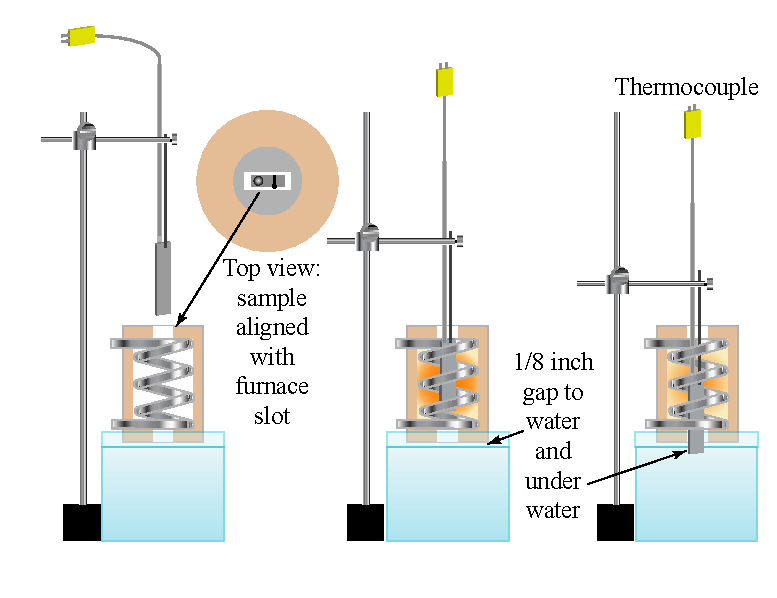
\includegraphics[width=250pt]{pics/diagram1.pdf}
\caption{Schematic experimental setup.
The thermocouple tip rests in a small depres-
sion in the top of the sample, which is sus-
pended by a Nichrome wire. Inset at left
shows crucial alignment of sample with the
rectangular slot at the bottom of the furnace.
In center frame, the entire sample is heated
to 1050$\degree$C and held for 5 minutes. At right,
the sample is lowered into the water, 
submerged 1/8 inch, to establish temperature
gradient (900$\degree$C at top) and held for 15 min-
utes. It may be necessary to replenish the
water supply due to evaporative losses. [2]}
\label{fig1}
\end{figure}

Heat the sample to 1050$\degree$C and hold it there for 5 minutes by adjusting the power dial. After 5 minutes we adjusted the clamps and lowered the sample 1/8 in into the water below. We then lowered the temperature to 900$\degree$C and kept it there for 15 minutes. After 15 minutes, we released the sample into the water and waited for it to cool.

\subsection{Metallographic Polishing and Etching.}
Take the sample over to the grinders and use the 120 grip paper grinder first. We placed the sample on the grider, turned on the water and grinded both sides of our sample. After the 120 grip paper, we moved to the 220 grip paper grinders and repeated the same procedures. We then moved on and used the hand grinded grid paper. Note we switched orientation by 90 $\degree$ until the orthogonal scratches disapeared. After the polishing, we handed the sample to the GSI in order for it to get etched down.

\subsection{Hardness Indentation test}

we performed a series of rockwell tests on our sample. these tests were evenly spaced out across the sample. Refer to figure 2 below to see where the tests where done on the sample.

\begin{figure}[H]
\centering
\begin{tikzpicture}
\draw[color = blue] (0,0) rectangle (2,8.1);
\draw[] (1,7.9) circle [radius=0.1];
\foreach \i in {0.5,1.0,...,7.5}
{
	\draw[color=red] (1,\i) circle [radius = 0.2];
}
\node at (-0.5,0.5) {1};
\node at (-0.5,1.0) {2};
\node at (-0.5,1.5) {3};
\draw[->] (-0.5,2) -- (-0.5,7);
\node at (-0.5,7.5) {16};
\node at (3,1) {100$\degree$C};
\node at (3,2.3) {260$\degree$C};
\node at (3,3.6) {420$\degree$C};
\node at (3,4.9) {580$\degree$C};
\node at (3,6.2) {740$\degree$C};
\node at (3,7.5) {900$\degree$C};
\draw[<->] (4,0) -- (4,8.1);
\node at (4.8,4) {2 inches};

\node at (-2,1.2) {\textcolor{red}{Martensite}};
\node at (-3,2.4) {\textcolor{red}{Martensite} + \textcolor{purple}{Pearlite}};
\node at (-2,3.6) {\textcolor{violet}{Pearlite} + \textcolor{green}{$\alpha$}};
\node at (-3,4.8) {\textcolor{red}{Martensite} + \textcolor{purple}{Pearlite} + \textcolor{green}{$\alpha$}};
\node at (-2,6.0) {\textcolor{red}{Martensite} + \textcolor{green}{$\alpha$}};
\node at (-2,7.2) {\textcolor{red}{Martensite}};

\draw[dashed] (-2,1.8) -- (2,1.8);
\draw[dashed] (-2,3) -- (2,3);
\draw[dashed] (-2,4.2) -- (2,4.2);
\draw[dashed] (-2,5.4) -- (2,5.4);
\draw[dashed] (-2,6.6) -- (2,6.6);
\end{tikzpicture}
\caption{The sample has 16 evenly spaced hardness tests on it. These tests are done in the middle of the sample starting from the bottom (1,2, etc) and ending at the top of the sample (16). The black circle represents the hole used to hang the sample in the furnace. The bottom part of the sample was dipped in water, hense the 100$\degree$C while the top was in the middle of the furnace at 900$\degree$C. The dashed lines show a rough estimate of the border between each transitional phase assuming the temperature gradient is linear. Note that \textcolor{green}{$\alpha$} in this case represents Ferrite (iron).}
\label{fig2}
\end{figure}

\subsection{Metallography}

We took the sample to the microscope room and viewed it under several different microscopes until we got decent looking pictures. The goal was to find the various phases that (martensite, pearlite, etc...).

\section{Experimental Results}
\begin{figure}[H]
\begin{tikzpicture}
\node at (5,5) {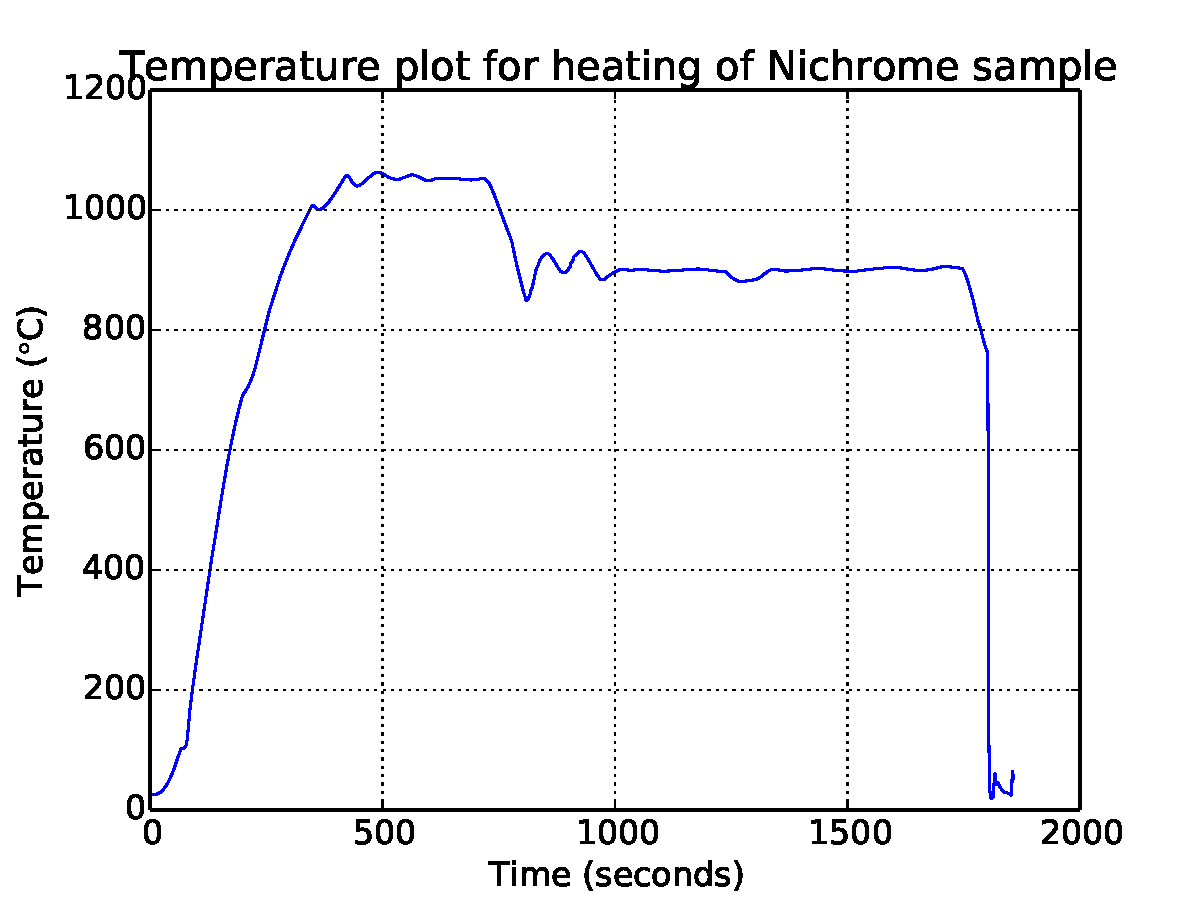
\includegraphics[width=325pt]{pics/fig1.pdf}};
\node at (15,5) {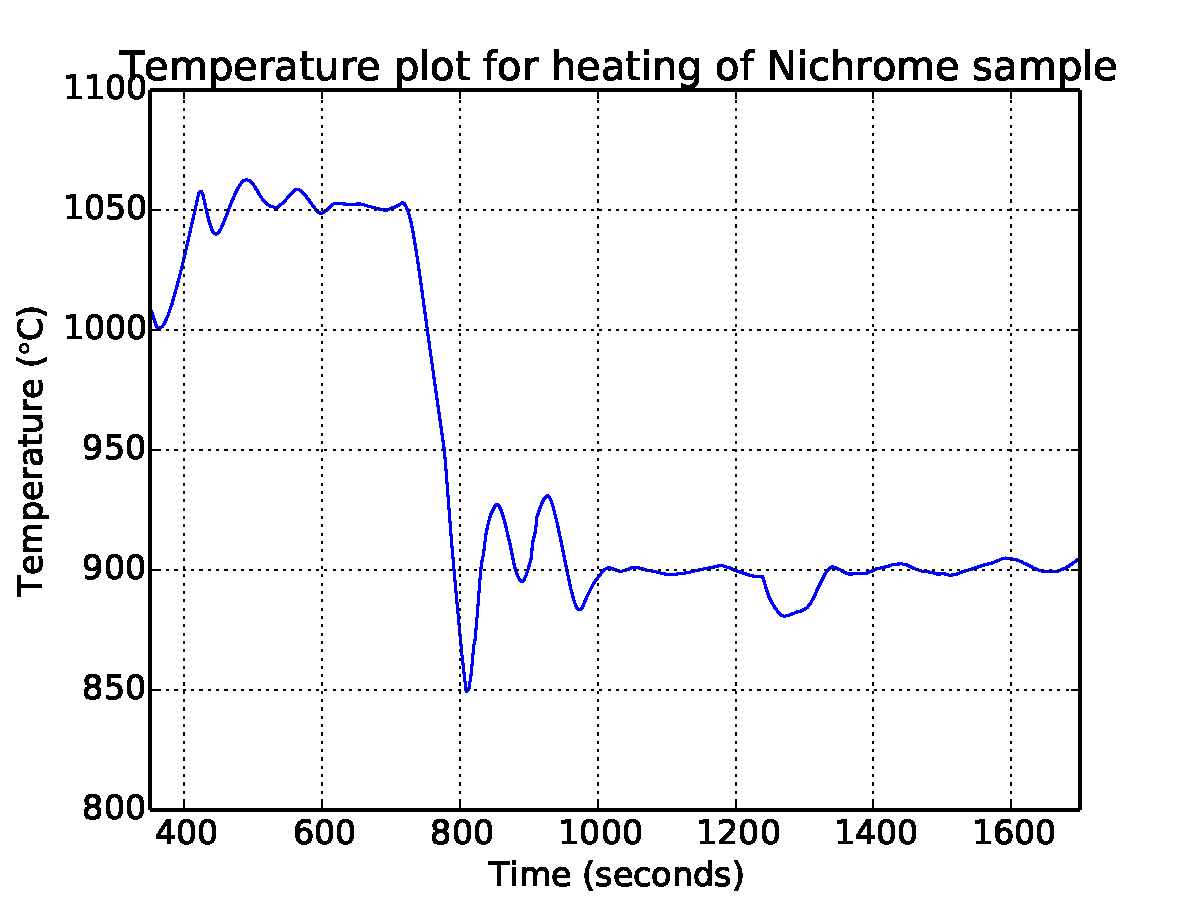
\includegraphics[width=250pt]{pics/fig2.pdf}};
\draw (2.3,6) rectangle (8.2,8);
\draw (8.2,8) -- (11.7,7.5);
\draw (8.2,6) -- (11.7,2.5);
\end{tikzpicture}
\caption{Time vs Temperature graph for data taken during heating. The transition from 1050$\degree$C to 900$\degree$C was a bit "bumpy" and not very smooth. The steep drop i temperature at the end was because our therostats tip fell into the water when we were in the process of releasing the sample in the water.}
\label{fig3}
\end{figure}

\begin{figure}[H]
\centering
\begin{tabular}{c || c | c | c}
\specialcell{Position \\ (figure 3)} & \specialcell{Major Load \\ (kg)} & \specialcell{Minor Load \\ (kg)} & \specialcell{Hardness \\ (HRA)} \\ \hline
1 & 60 & 10 & 82.0 \\ \hline
2 & 60 & 10 & 80.9 \\ \hline
3 & 60 & 10 & 73.2 \\ \hline
4 & 60 & 10 & 66.0 \\ \hline
5 & 60 & 10 & 72.9 \\ \hline
6 & 60 & 10 & 61.4 \\ \hline
7 & 60 & 10 & 65.7 \\ \hline
8 & 60 & 10 & 65.0 \\ \hline
9 & 60 & 10 & 64.8 \\ \hline
10 & 60 & 10 & 62.9 \\ \hline
11 & 60 & 10 & 62.1 \\ \hline
12 & 60 & 10 & 59.8 \\ \hline
13 & 60 & 10 & 58.0 \\ \hline
14 & 60 & 10 & 61.4 \\ \hline
15 & 60 & 10 & 66.2 \\ \hline
16 & 60 & 10 & 79.5 \\ \hline
\end{tabular}
\caption{Refer to Figure \textcolor{blue}{\ref{fig2}} to understand the position references made in the table above.}
\label{fig4}
\end{figure}

\begin{figure}[H]
\centering
\begin{tikzpicture}
\node at (0,10) {\fbox{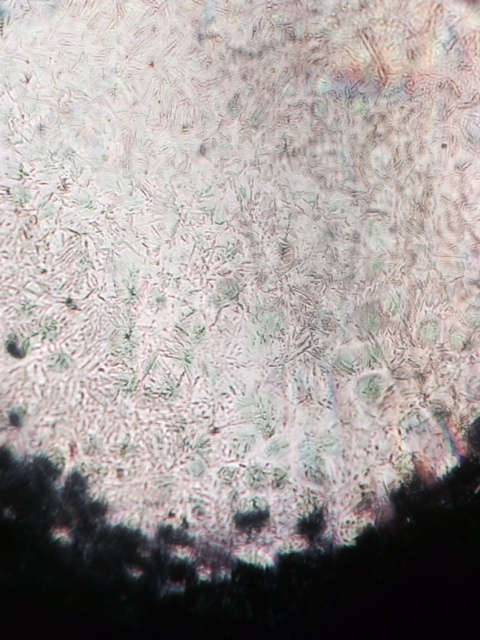
\includegraphics[width=100pt]{pics/image1.jpeg}}};
\node at (4,10) {\fbox{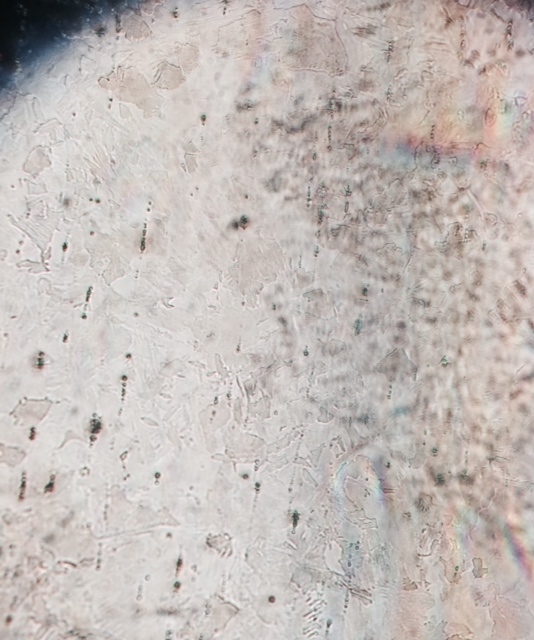
\includegraphics[width=100pt]{pics/image2.jpeg}}};
\node at (8,10) {\fbox{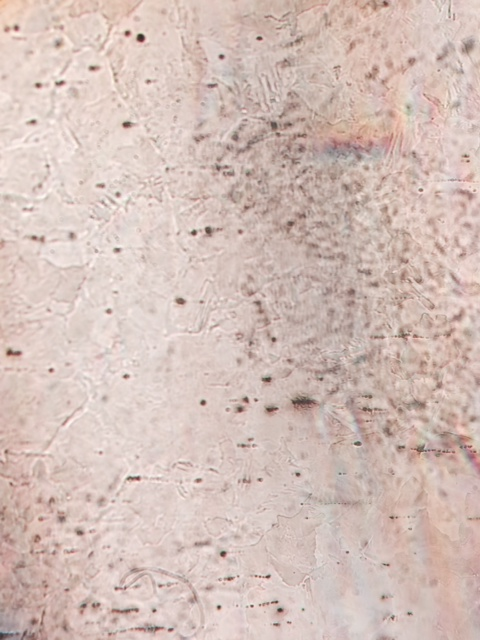
\includegraphics[width=100pt]{pics/image3.jpeg}}};
\node at (12,10) {\fbox{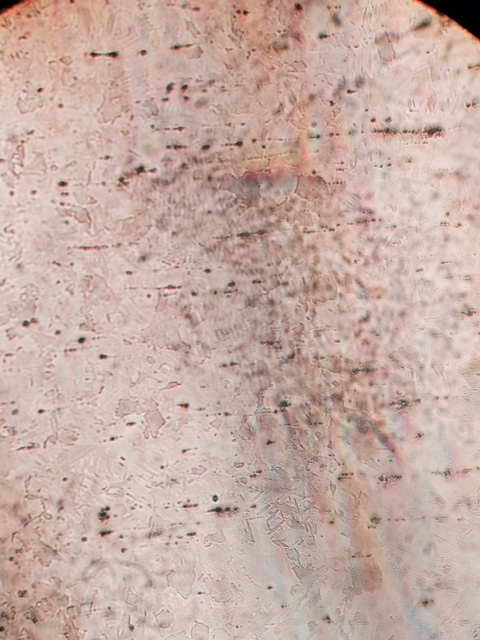
\includegraphics[width=100pt]{pics/image4.jpeg}}};
\node at (16,10) {\fbox{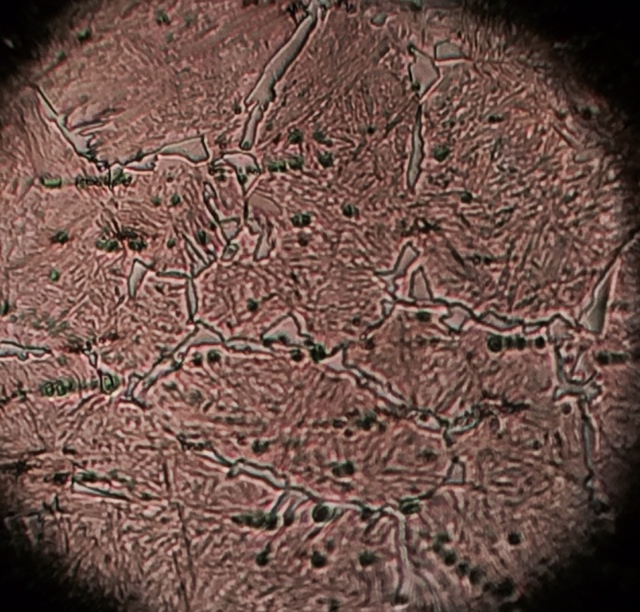
\includegraphics[width=100pt]{pics/image5.jpeg}}};

\node at (0,7) {Position 1};
\node at (4,7) {Position 5};
\node at (8.0,7) {Position 8};
\node at (12.5,7) {Position 12};
\node at (16,7) {Position 16};
\end{tikzpicture}
\caption{The 5 images taken for the microstructure of the sample. The pictures turned out very bad because of the way they were taken (cell phone camera held up to microscope). Pictures are high resolution, so zoom in to see more detail. Refer to Figure \textcolor{blue}{\ref{fig2}} to find a reference for the positions.}
\label{fig5}
\end{figure}

\section{Discussion}

\begin{description}[style = nextline]
\item[1) For each of the five (5) different microstructures evident in your results, draw a representative cooling curve on a TTT diagram corresponding to the thermal history associated with the specific area of the sample where the microstructure was observed. Use a separate TTT diagram for each of the five cooling curves, but show them all at the same scale. Verify the phases present in each microstructure and compare to your cooling curves. Specify the order in which the phases appeared, and refer to the phase diagram as necessary to validate your conclusions.]

Refer to figure 6 below.

\begin{figure}[H]
\centering
\begin{tikzpicture}
\node at (5,5) {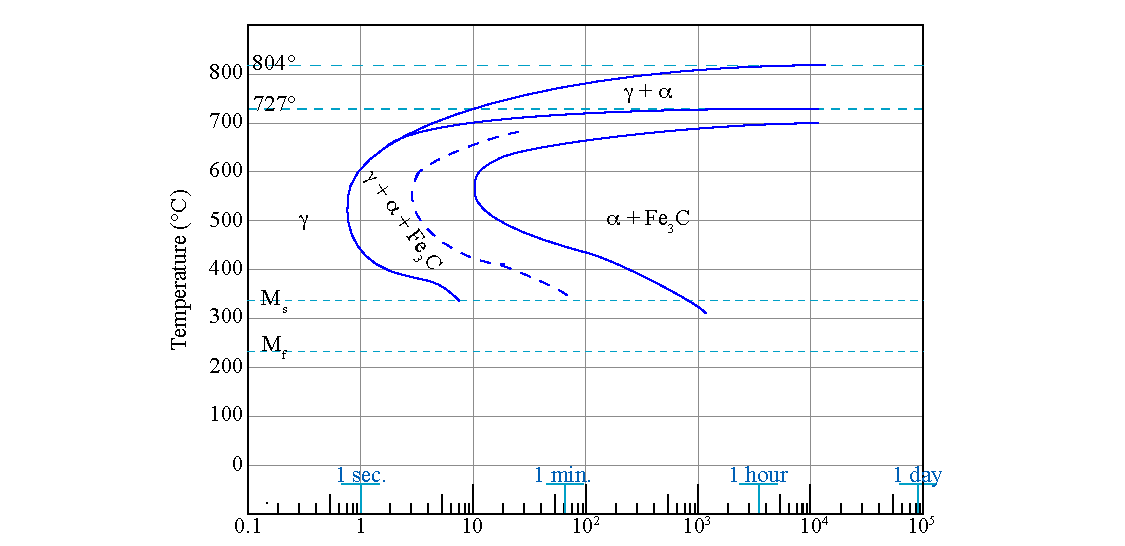
\includegraphics[width=500pt]{pics/diagram22.pdf}};
\node at (5,9.5) {\textbf{\large{TTT curve for all five microstructures present on sample}}};
\draw[->,color=red] (1,8.9) -- (1.1,2.75);
\draw[->,color=red] (1.1,2.75) -- (7,2.75);
\node at (3,2.5) {\color{red}{M}};

\draw[->,color=violet,thick] (1.1,4.4) -- (7,4.4);
\node at (3,4.2) {\color{red}{M} + \color{purple}{P}};

\draw[->,color=orange,thick] (1.05,7.3) -- (7,7.3);
\node at (1.9,7.15) {\color{green}{$\alpha$} + \color{purple}{P}};

\draw[->,color=green,thick] (1.0,7.5) -- (7,7.5);
\node at (1.9,7.7) {\color{red}{M} + \color{green}{$\alpha$} + \color{purple}{P}};

\draw[->,color=pink,thick] (1.0,7.9) -- (7,7.9);
\node at (1.9,8.1) {\color{red}{M} + \color{green}{$\alpha$}};

\draw[->] (7,7.9) -- (7,2);

%legend
\draw[color=black] (12,3) rectangle (15,8);

\draw[color=red,line width = 1pt] (12.1,7.5) -- (12.5,7.5);
\node at (13.7,7.5) {\color{red}{M}};

\draw[color=violet,line width = 1pt] (12.1,6.5) -- (12.5,6.5);
\node at (13.7,6.5) {\color{red}{M} + \color{purple}{P}};

\draw[color=orange,line width = 1pt] (12.1,5.5) -- (12.5,5.5);
\node at (13.7,5.5) {\color{purple}{P} + \color{green}{$\alpha$}};

\draw[color=green,line width = 1pt] (12.1,4.5) -- (12.5,4.5);
\node at (13.5,4.5) {\color{red}{M} + \color{purple}{P} + \color{green}{$\alpha$}};

\draw[color=pink,line width = 1pt] (12.1,3.5) -- (12.5,3.5);
\node at (13.5,3.5) {\color{red}{M} + \color{green}{$\alpha$}};

% special locations
\node at (1.1,2.4) {\textbf{(1)}};
\node at (7.3,2.4) {\textbf{(2)}};
\draw[<->] (0,0.8) -- (7,0.8);
\node at (3,0.5) {15 minutes};
\end{tikzpicture}
\caption{All five phases were plotted in the figure above. Note that M stands for Martensite, P for Pearlite, and $\alpha$ for ferrite. Initially our sample temperature is at 1100$\degree$C. The bottom 1/4 inch of the sample is then dipped into water. This occurs at location \textbf{(1)} in the figure. The bottom piece of the sample immediately turns into martensite as is evident in the figure. The top of the sample is then reduced to a temperature of 900$\degree$C; this creates a (hopefully linear) temperature gradient across the sample which is illustrated in Figure \textcolor{blue}{\ref{fig2}}. The various temperatures across the sample now create different phases according to the TTT curve above. After 15 minutes we hit point \textbf{(2)} where the whole sample is dropped into water.}
\label{fig6}
\end{figure}

We can compare our microstructure images in Figure \textcolor{blue}{\ref{fig5}} with where we think the changes should actually occur in Figure \textcolor{blue}{\ref{fig2}}. Although most of our images taken of the microstructure turned out very bad, looking at the image at position 1, you can tell that this microstructure is infact Martensite because of the lines present. Also the image at position 16 shows what looks like Martensite + ferrite microstructure because of the lines and new grains that have formed.

Using the cooling curve above, we can figure out what order the microstructures occured. Initially you have martensite that occurs when the bottom piece of the sample is dipped in water. After that the $\alpha$ microstructure starts to form (green line in figure) followed by Pearlite (green, orange, and pink lines).

\item[2) Make a plot of hardness versus distance from the 900$\degree$C end of the sample. Use your hardness data to rank martensite, ferrite, and pearlite from the hardest to the softest. Support your results by discussing the nature of the microstructure, crystal structure, and chemical bonding associated with all three phases (martensite, ferrite, and carbide).]

Looking at the figure below and comparing it with Figure \textcolor{blue}{\ref{fig2}}, we can compare the hardness of various phases present. The length of the sample in the figure below is measured from the top of the sample (900$\degree$C) to the bottom of the sample (100$\degree$C). 

\begin{enumerate}
\item Martensite
\item Martensite + Pearlite
\item Pearlite + $\alpha$
\item Martensite + Pearlite + $\alpha$
\item Martensite + $\alpha$
\end{enumerate}
1 represents the strongest while 5 represents the weakest of the phases. Note $\alpha$ stands for Ferrite (iron).
\begin{figure}[H]
\centering
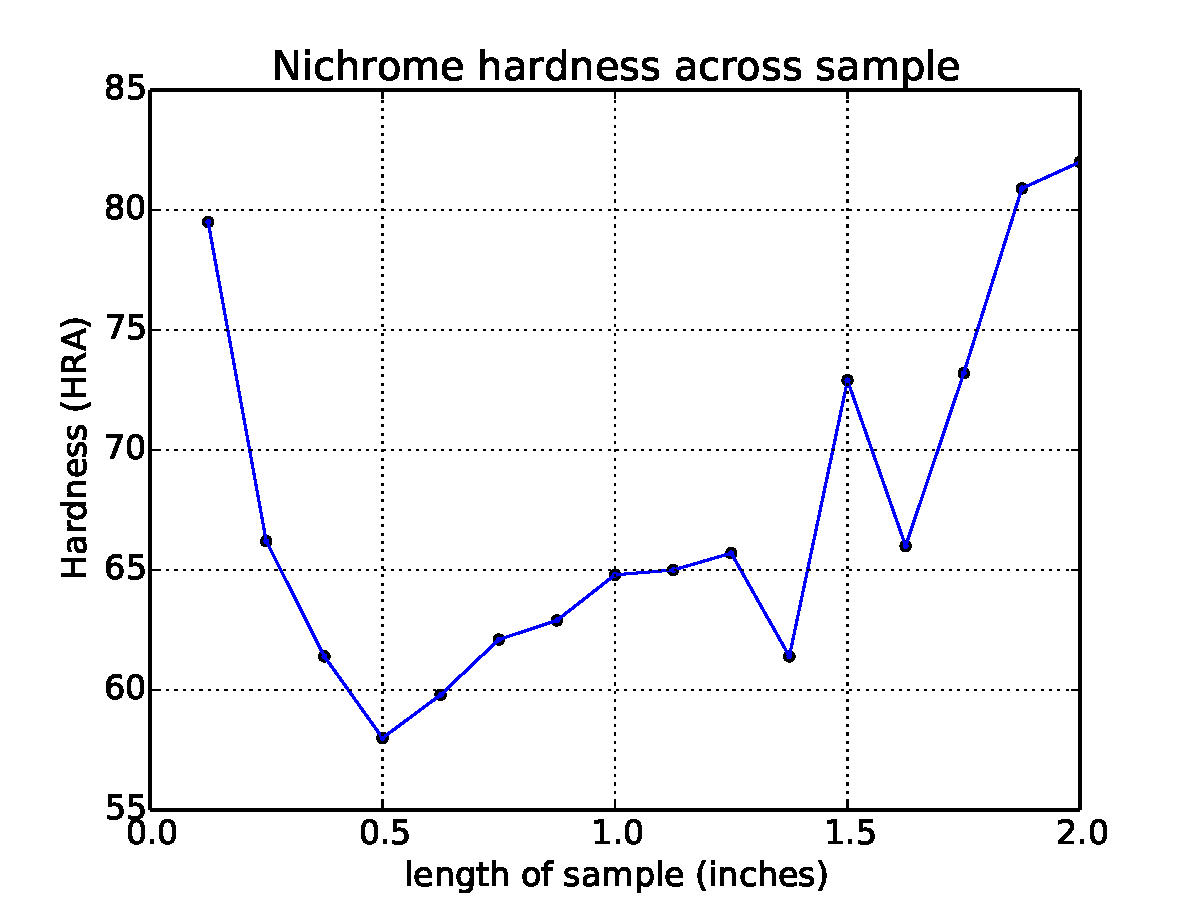
\includegraphics[width=300pt]{pics/fig3.pdf}
\caption{"Nichrome hardness as a function of length across the sample when heated up to 900 degrees. 0 inches starts at position 16 and 2 inches ends at position 0 on Figure \textcolor{blue}{\ref{fig2}}. Rankings of the phases is below. The weird spiking at around 1.5 inches was most likely because the sample was not perfectly dipped 1/8 inch into the water, but was instead dipped and moved around (up and down) in the water until an acceptable position was achieved.}
\label{fig7}
\end{figure}

If we look at the microstructure of the phases, we can see that the figure above makes sense. If martensite were to form, that means that no carbon can precipiate as $\text{Fe}_3$C and as a result there is no nucleation or growth of pearlite. Instead the structure turns into a bct lattice trapping the randomly dstributed carbon. Because the carbon atoms can't diffuse out in time, martensite ends up having the largest hardness. Pearlite is a two phase structure that contains lamellar lines of ferrite and cementite phase (a carbide, $\text{Fe}_3$C). Ferrite is a BCC structure that can have at maximum 0.02\% carbon in it while cementite is a FCC structure than contains up to 2\% carbon in Fe.

\item[3) Does the transformation of austenite into ferrite begin at the austenite grain boundaries and propagate inward, or does it begin inside the grains and propagate outward toward the boundaries? Include a sketch of the microstructure from the appropriate part of the specimen illustrating the answer to this question. Explain.]

Looking at the image for position 16 in Figure \textcolor{blue}{\ref{fig5}} it looks like the transformation is forming at the grain boundaries vs inside the grains. According to the textbook on page 306 [1] heterogeneous nucleation which occurs at the structural imperfections, grain boundaries, are must more common. This is because the imperfections, grain boundaries, reduce the surface energy associated with forming the new phase.

\item[4)How could a structure containing only ferrite and martensite be produced in a 1045 steel specimen? Illustrate on a TTT diagram.]

Looking at Figure \textcolor{blue}{\ref{fig6}} we can see that the pink line is indeed in a Martensite + ferrite phase. Holding the temperature anywhere between 727$\degree$C and 804$\degree$C will form a Martensite + ferrite phase according to the 1045 steel TTT diagram.

\item[5) Could you heat treat a 1045 steel specimen so that it contains only ferrite? Describe how this can be achieved, or explain why it cannot be done.]

Looking at the TTT diagram in Figure \textcolor{blue}{\ref{fig6}} we can see that it would not be possible to form a sample with pure ferrite. This is because austenite cannot be quenched to form just $\alpha$ phase, but can only be quenched to form martensite.

\item[6) Why isn't martensite on the Fe-$\text{Fe}_3$C phase diagram of Fig. 1? Why doesn't its absence from the phase diagram prevent it from being an important engineering material?]

Martensite is not an equilibrium phase and as such does not appear on the phase diagram; it is a phase that is formed through a diffusionless process meaning that the atoms in the lattice move a very small distance in unison. A term for this type of movement is 'military transformation'. Although not in the phase diagram, martensite is a very strong material, although brittle, that can be used for many applications. If tempered, the phase becomes even stronger.
\end{description}
%----------------------------------------------------------------------------------------
%	SECTION 4
%----------------------------------------------------------------------------------------

\section{Conclusions}
As a result of this investigation, the following conclusions can be drawn.
\begin{enumerate}
\item A ranking of phase hardness was achieved (see Figure \textcolor{blue}{\ref{fig7}}).
\item Using the images of the phase microstructures, we were able to verify when certain phases appeared based on a TTT curve generated in Figure \textcolor{blue}{\ref{fig6}}
\item The microscopes used to take images of the phases did not work very well and gave us focusing problems.
\end{enumerate}

%----------------------------------------------------------------------------------------
%	SECTION 5
%----------------------------------------------------------------------------------------

\section{References}
\begin{enumerate}
\item James F. Shackelford, Introduction to Materials Science for Engineers, Seventh Edition, Pearson Higher 
Education, Inc., Upper Saddle River, New Jersey (2009).
\item Gronsky, Ron. Lab 05 Manual: Heat Treatment of Steel. Berkeley: Ronald Gronsky, 2014. Web.
\end{enumerate}

%----------------------------------------------------------------------------------------
%	SECTION 6
%----------------------------------------------------------------------------------------

% Nothing right now

%----------------------------------------------------------------------------------------
%	BIBLIOGRAPHY
%----------------------------------------------------------------------------------------

\bibliographystyle{apalike}

\bibliography{sample}

%----------------------------------------------------------------------------------------


\end{document}

